\documentclass[12pt,a4paper]{article}
\usepackage[ngerman]{babel}
\usepackage[utf8]{inputenc}
\usepackage[unicode=true,bookmarks=false,bookmarksopen=true]{hyperref}

\usepackage{xcolor}
\usepackage{graphicx}
\usepackage{tikz}

\usepackage{listings}

\def\checkmark{\tikz\fill[scale=0.4](0,.35) -- (.25,0) -- (1,.7) -- (.25,.15) -- cycle;}

\definecolor{pGreen}{rgb}{0.44, 0.71, 0}
\definecolor{nRed}{rgb}{0.74, 0, 0}

\title{ORES Custom Documentation VI}
%\author{Tom Gülenman}
\date{}
\begin{document}
\maketitle
\textit{Disclaimer: No guarantee for the correctness of information / explanations / sources is given.}\\
%
\section*{Goals}
\begin{enumerate}
\item Metrics List: Create Table as a general quick-view
\item Metrics: which combinations are particularly useful, which are nonsensical?
\begin{itemize}
\item Ask for documentation on IRC (\checkmark)
\item Logically exclude combinations?
\item Document outputs
\end{itemize}
\item Recent Changes filter classes: how are edits assigned to them?
\begin{itemize}
\item Also ask for documentation on IRC \checkmark
\item Which metrics are included in the process? \checkmark
\item How are the metrics (precision, recall, threshold) included in the associated API calls? What do the (GET?)-Requests look like?
\end{itemize}
\item Take a closer look at the Threshold Plot for Logistic Regression (\href{http://www.scikit-yb.org/en/latest/api/classifier/threshold.html}{Link})
\begin{itemize}
\item What is the meaning of the areas around the curves?
\item What is queue rate exactly?
\end{itemize}
\item Take a closer look at the Swagger API Documentation
\item \colorbox{red}{ !!! } Improve knowledge of ORES Docs and foremost the metrics
\end{enumerate}
%
%
%
\newpage
\section{Metrics List: Table}
%TODO
%
%
%
\section{Metrics combinations}
example: \url{https://ores.wikimedia.org/v3/scores/enwiki/?models=damaging&model_info=statistics.thresholds.true.%27maximum%20!precision%20@%20precision%20%3E=%200.9%27}
%TODO
%TODO also see https://www.mediawiki.org/wiki/ORES/Thresholds -> worked example
%
%
%
\section{Recent Changes Quality Prediction Filters}
The Recent Changes quality prediction filters are a helpful tool in varying the precision and recall of catching damaging edits. They can be applied on the Recent changes site (\href{https://en.wikipedia.org/wiki/Special:RecentChanges?hidebots=1&hidecategorization=1&hideWikibase=1&limit=50&days=7&urlversion=2}{Link}).\\
\\
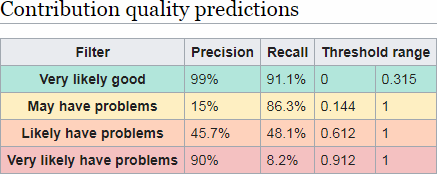
\includegraphics[scale=0.85]{resources/6/RCFilters}\\
{\href{https://en.wikipedia.org/wiki/Special:ORESModels}{Wikipedia Source}\\
\\
To put those numbers into context: we can expect that, for example, the \textit{Likely have problems} filter will be right about $45.7\%$ of the time, classifying a contribution as damaging while catching $48.1\%$ of problem edits.\\
To better understand threshold ranges it's helpful to also take a look at the following graphic:\\
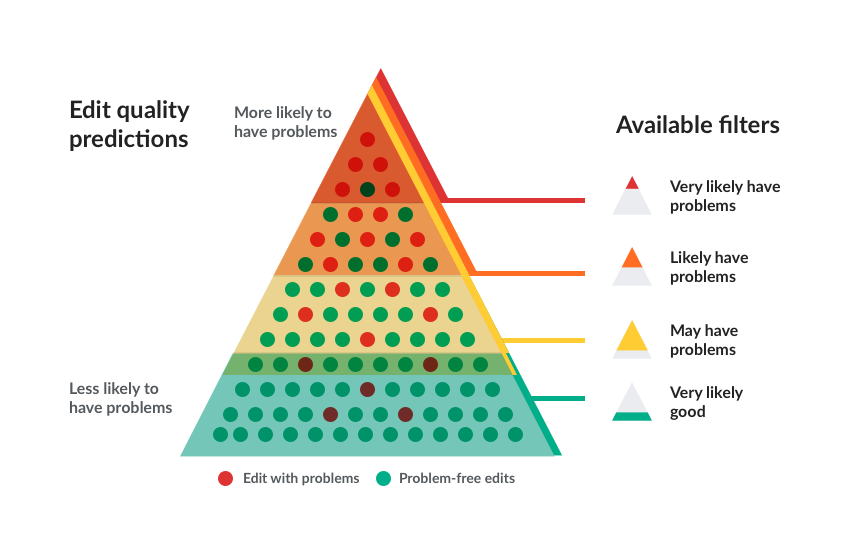
\includegraphics[scale=0.5]{resources/6/RC-quality-filters-diagram}\\
\href{https://upload.wikimedia.org/wikipedia/commons/e/e8/RC-quality-filters-diagram.png}{Wikimedia Source}\\
%TODO explanation
%TODO Highlighting?
\end{document}